\usepackage[english] {babel}
\usepackage[T1]      {fontenc}

\usepackage{amsmath, amsfonts, graphicx}
\usepackage{bibunits, tikz}
\usepackage{listings}
\usepackage{perpage}
\usepackage{courier}
\MakePerPage{footnote}

\usetheme{progressbar}

\AtBeginSection{\frame{\sectionpage}}

\defbeamertemplate{section page}{mine}[1][]{%
  \begin{centering}
    \vskip1em\par
    \begin{beamercolorbox}[sep=12pt,center]{part title}
      \usebeamerfont{section title}\insertsection\par
    \end{beamercolorbox}
  \end{centering}
}

\setbeamersize
  {text margin left=1em, text margin right=1em}

\title
  [Understanding Random Forests - Marc Garcia]
  {\Large{Understanding Random Forests}}

\author
  [Marc Garcia]
  {Marc Garcia}

\date
  {PyData Madrid - April 9th, 2016}


\begin{document}

\maketitle

\setbeamertemplate{section page}[mine]

\lstset{breakatwhitespace=true,
        language=Python,
        columns=fullflexible,
        keepspaces=true,
        breaklines=true,
        tabsize=4, 
        showstringspaces=false,
        extendedchars=false,
        numbers=none,
        basicstyle=\tiny\ttfamily,
        keywordstyle=\color{blue},
        stringstyle=\color{red},
        commentstyle=\color{green},
        morecomment=[l][\color{magenta}]{\#}
}


%\begin{frame}{Overview}
%    \tableofcontents
%\end{frame}

\section{Introduction}

\begin{frame}{About me: @datapythonista}
    
\includegraphics[scale=.5]{images/about_me}

    \begin{columns}
     \begin{column}{.49\textwidth}
        \begin{itemize}
            \Large
            \item \textbf{Python} programmer since 2006
            \item \textbf{Master in AI} from UPC
        \end{itemize}
     \end{column}
    
     \begin{column}{.49\textwidth}
        \begin{itemize}
            \Large
            \item Working for \textbf{Bank of America}
            \item http://datapythonista.github.io
        \end{itemize}
     \end{column}
    \end{columns}
\end{frame}


\begin{frame}{Overview: Understanding Random Forests}
    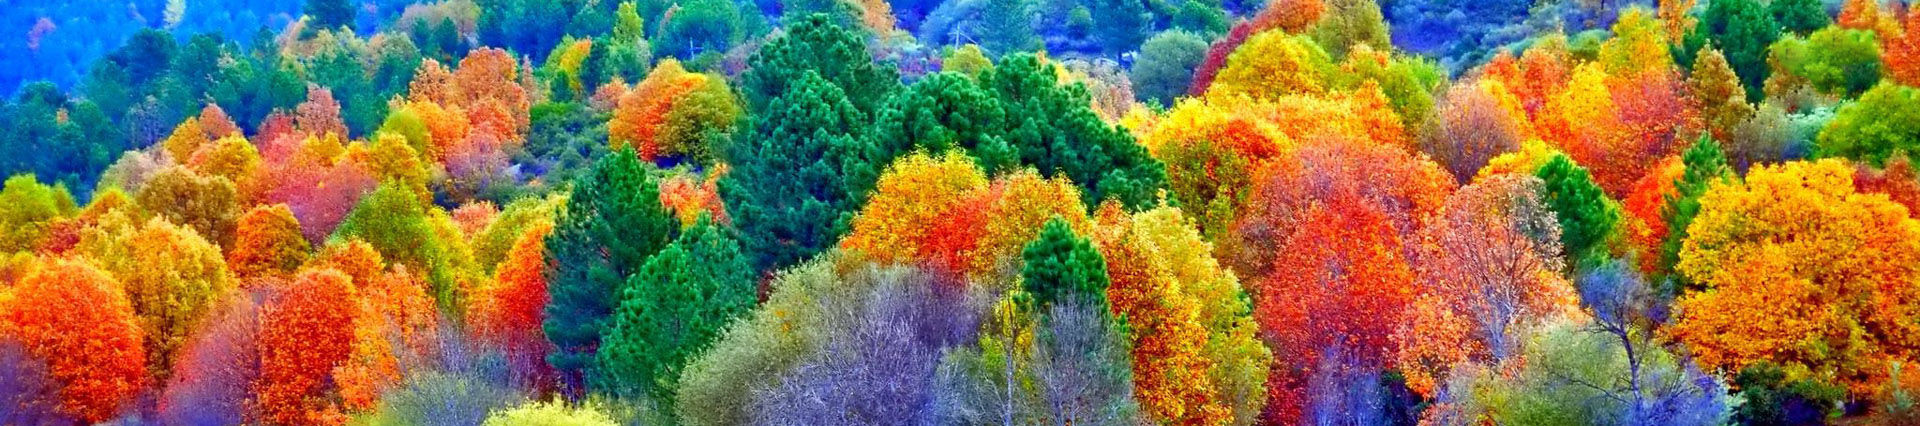
\includegraphics[scale=.9]{images/trees_colors}

    \begin{columns}
     \begin{column}{.49\textwidth}
        \begin{itemize}
            \Large
            \item How \textbf{decision trees} work
            \item \textbf{Training} Random Forests
        \end{itemize}
     \end{column}
    
     \begin{column}{.49\textwidth}
        \begin{itemize}
            \Large
            \item Practical \textbf{example}
            \item Analyzing model \textbf{parameters}
        \end{itemize}
     \end{column}
    \end{columns}
\end{frame}


\section{How decision trees work}
%%%%%%%%%%%%%%%%%%%%%%%%

\begin{frame}[fragile]{Using a decision tree}
    \begin{columns}
     \begin{column}{.49\textwidth}
        Simple example:
        \begin{itemize}
            \item Event attendance: binary classification
            \item 2 explanatory variables: age and distance
        \end{itemize}
     \end{column}
    
     \begin{column}{.49\textwidth}
        \lstinputlisting{src/04_plot_cart.py}
     \end{column}
    \end{columns}
\end{frame}

\begin{frame}[fragile]{Data visualization}
    \begin{center}
        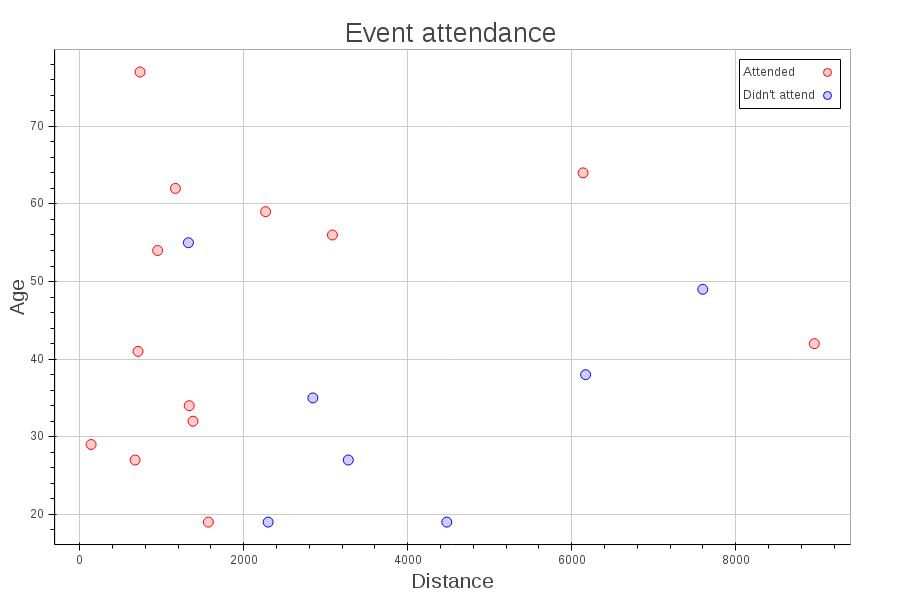
\includegraphics[scale=.25]{images/event_attendance}
    \end{center}
\end{frame}

\begin{frame}[fragile]{Decision boundary visualization}
    \begin{center}
        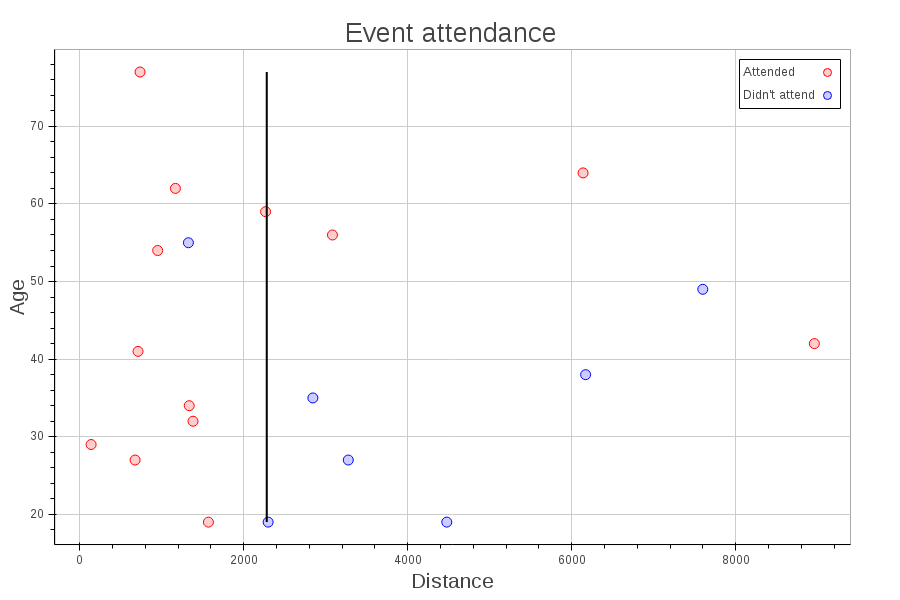
\includegraphics[scale=.25]{images/decision_tree_plot_1}
    \end{center}
\end{frame}

\begin{frame}[fragile]{Decision boundary visualization}
    \begin{center}
        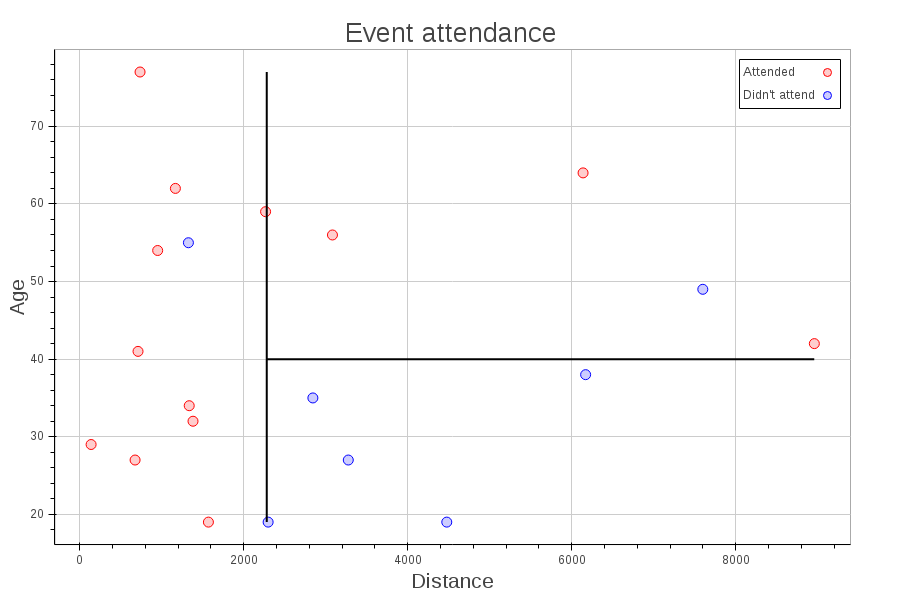
\includegraphics[scale=.25]{images/decision_tree_plot_2}
    \end{center}
\end{frame}

\begin{frame}[fragile]{Decision boundary visualization}
    \begin{center}
        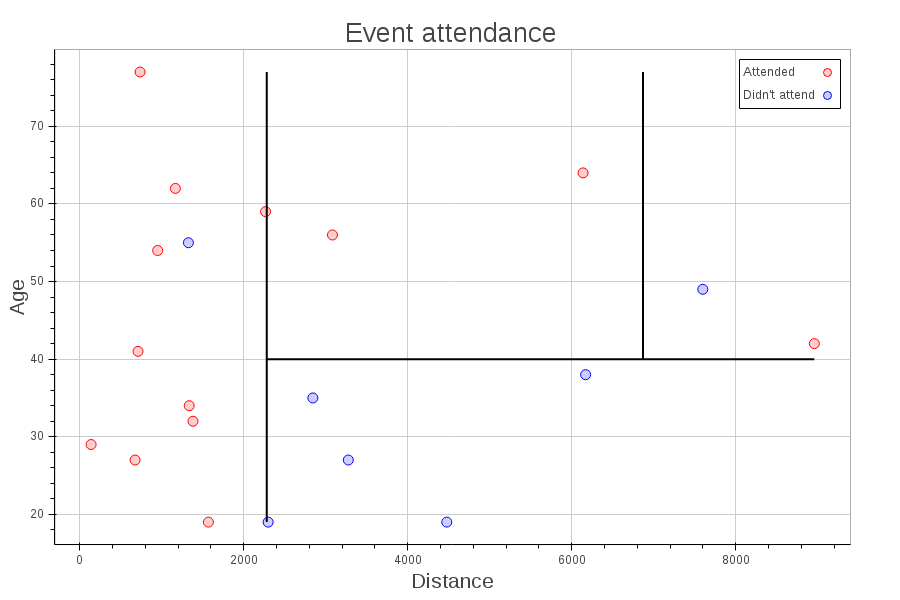
\includegraphics[scale=.25]{images/decision_tree_plot_3}
    \end{center}
\end{frame}

\begin{frame}[fragile]{Decision boundary visualization}
    \begin{center}
        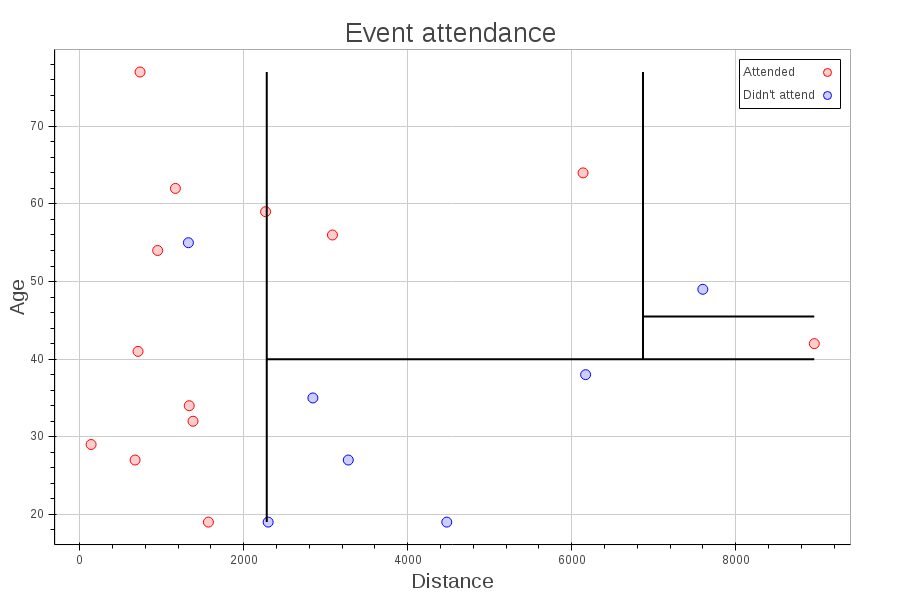
\includegraphics[scale=.25]{images/decision_tree_plot_4}
    \end{center}
\end{frame}

\begin{frame}[fragile]{Decision boundary visualization}
    \begin{center}
        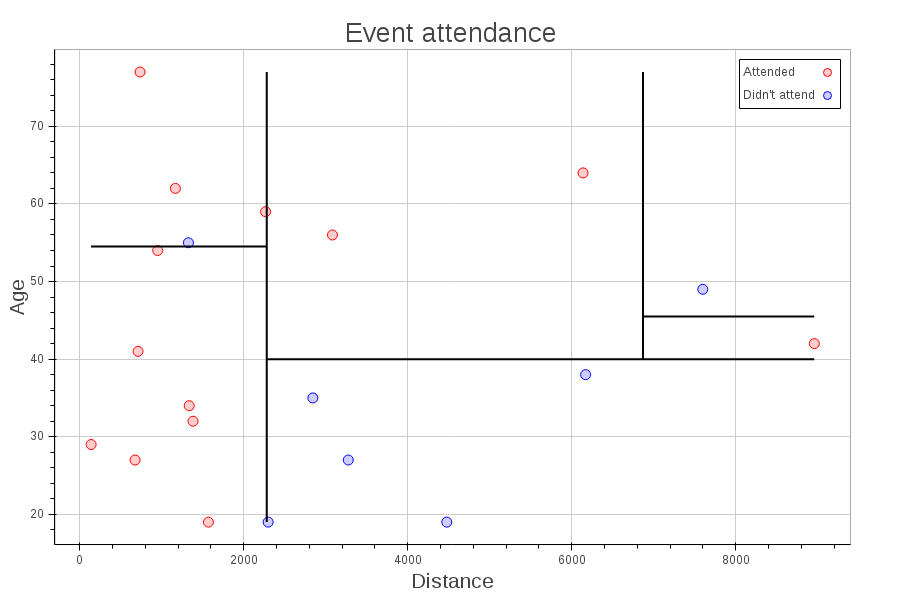
\includegraphics[scale=.25]{images/decision_tree_plot_5}
    \end{center}
\end{frame}

\begin{frame}[fragile]{Decision boundary visualization}
    \begin{center}
        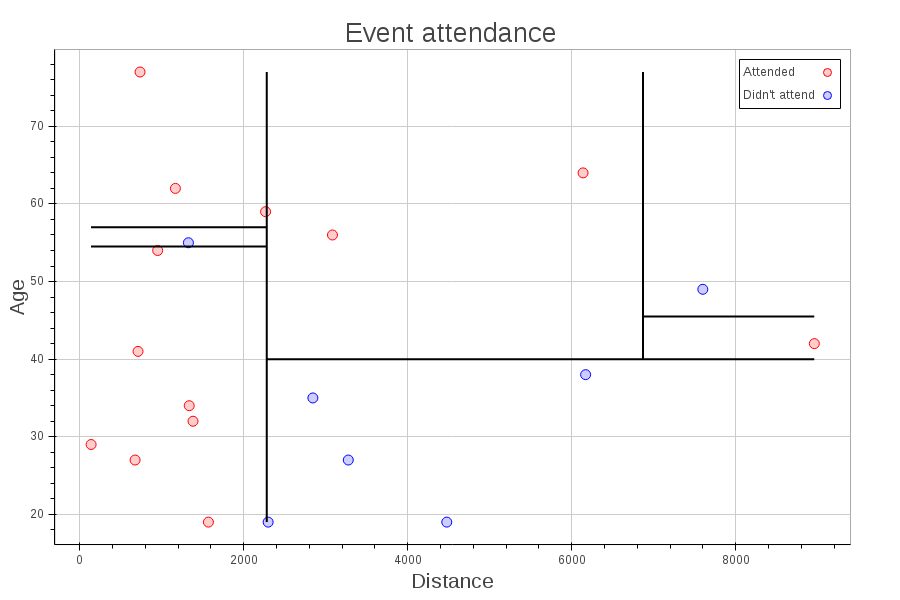
\includegraphics[scale=.25]{images/decision_tree_plot_6}
    \end{center}
\end{frame}


\begin{frame}{How is the model?}
    \begin{columns}
     \begin{column}{.49\textwidth}
        \lstinputlisting{src/05_cart_ifs.py}
     \end{column}
    
     \begin{column}{.49\textwidth}
        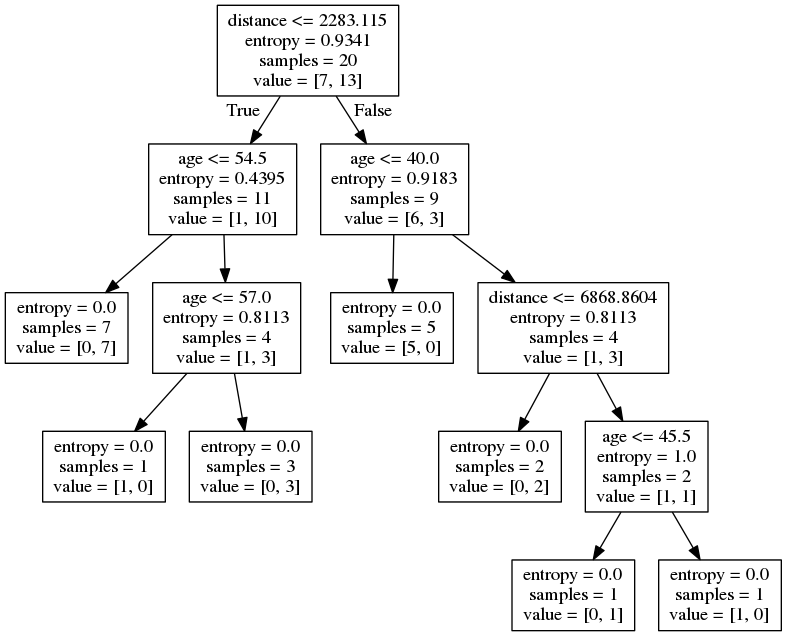
\includegraphics[scale=.25]{images/tree}
     \end{column}
    \end{columns}
\end{frame}


\begin{frame}[fragile]{Training: Basic algorithm}
    \lstinputlisting{src/07_train_cart.py}
\end{frame}

\begin{frame}[fragile]{Best split}
    \textbf{Candidate split 1}
    \begin{tabular}{ll|lllllllllll}
    \toprule
    age & 18 & 19 & 21 & 27 & 29 & 34 & 38 & 42 & 49 & 54 & 62 & 64 \\
    \midrule
    attended &  F &  F &  T &  F &  T &  T &  F &  T &  F &  T &  T &  T \\
    \bottomrule
    \end{tabular}

    \begin{center}
        \begin{tabular}{lll}
        \toprule
        Split & True & False \\
        \hline
        \midrule
        Left & 0 & 1 \\
        Right & 7 & 4 \\
        \bottomrule
        \end{tabular}
    \end{center}


    \textbf{Candidate split 2}
    \begin{tabular}{lll|llllllllll}
    \toprule
    age & 18 & 19 & 21 & 27 & 29 & 34 & 38 & 42 & 49 & 54 & 62 & 64 \\
    \midrule
    attended &  F &  F &  T &  F &  T &  T &  F &  T &  F &  T &  T &  T \\
    \bottomrule
    \end{tabular}

    \begin{center}
        \begin{tabular}{lll}
        \toprule
        Split & True & False \\
        \hline
        \midrule
        Left & 0 & 2 \\
        Right & 7 & 3 \\
        \bottomrule
        \end{tabular}
    \end{center}

\end{frame}

\begin{frame}[fragile]{Best split algorithm}
    \lstinputlisting{src/08_best_split.py}
\end{frame}

\begin{frame}[fragile]{Entropy}
    For a given \textbf{subset}\footnote{Note that for pure splits it's assumed that 0 \cdot \log_{2} 0 = 0}:
    \begin{equation}
        entropy = - Pr_{attending} \cdot \log_{2} Pr_{attending} - Pr_{\neg attending} \cdot \log_{2} Pr_{\neg attending}
    \end{equation}
    \begin{center}
        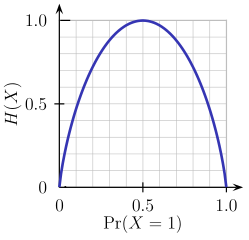
\includegraphics[scale=.5]{images/entropy}
    \end{center}
\end{frame}

\begin{frame}[fragile]{Entropy algorithm}
    \lstinputlisting{src/09_entropy.py}
\end{frame}

\begin{frame}[fragile]{Information gain}
    For a given \textbf{split}:
    \begin{equation}
        information\_gain = entropy_{parent} - \left( \frac{items_{left}}{items_{total}} \cdot entropy_{left} + \frac{items_{right}}{items_{total}} \cdot entropy_{right} \right)
    \end{equation}

\end{frame}

\section{Practical example}

\begin{frame}{Etsy dataset}
    \begin{columns}
     \begin{column}{.44\textwidth}
        \begin{itemize}
            \item Features:
            \begin{itemize}
                \item Feedback (number of reviews)
                \item Age (days since shop creation)
                \item Admirers (likes)
                \item Items (number of products)
            \end{itemize}
            \item Response variable:
            \begin{itemize}
                \item Sales (number)
            \end{itemize}
            \item Samples:
            \begin{itemize}
                \item 58,092
            \end{itemize}
            \item Source:
            \begin{itemize}
                \item www.bigml.com
            \end{itemize}
        \end{itemize}
     \end{column}

     \begin{column}{.54\textwidth}
        \begin{center}
            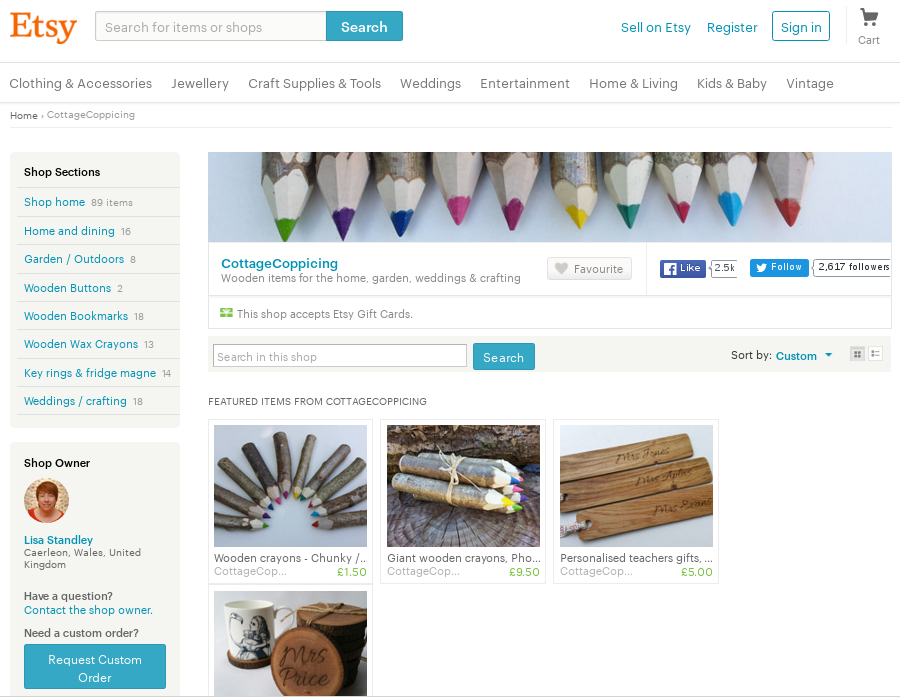
\includegraphics[scale=.22]{images/etsy_screenshot}
        \end{center}
     \end{column}
    \end{columns}
\end{frame}


\begin{frame}[fragile]{Features distribution}
    \begin{columns}
     \begin{column}{.49\textwidth}
        \begin{center}
            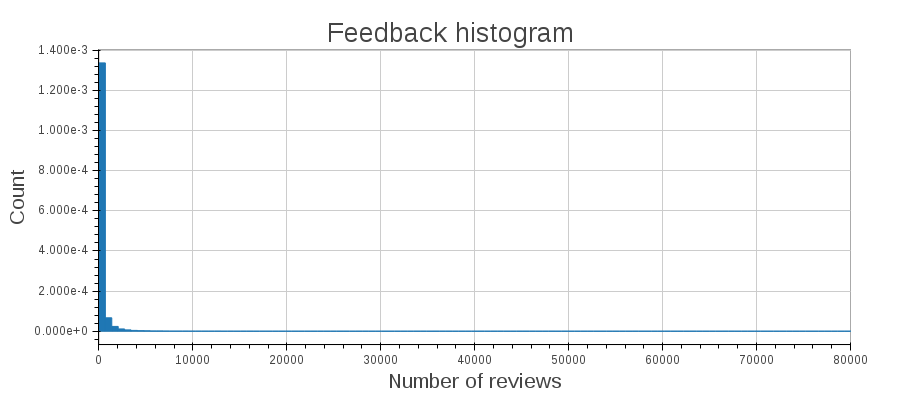
\includegraphics[scale=.18]{images/histogram_feedback}
        \end{center}
        \newline{}
        \begin{center}
            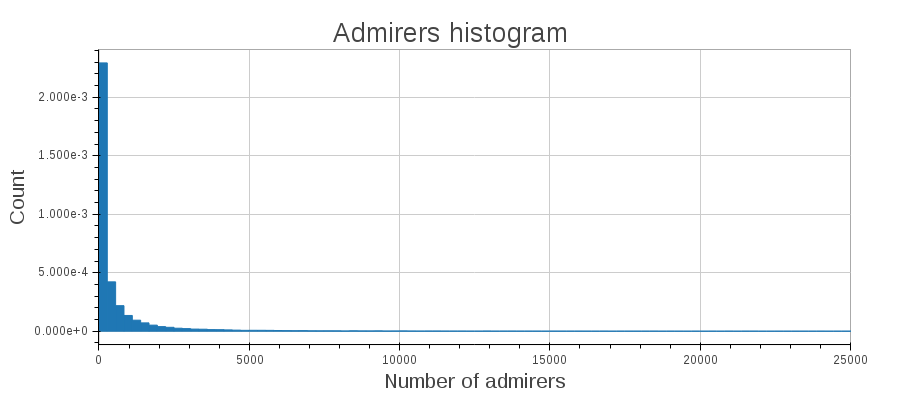
\includegraphics[scale=.18]{images/histogram_admirers}
        \end{center}
     \end{column}
    
     \begin{column}{.49\textwidth}
        \begin{center}
            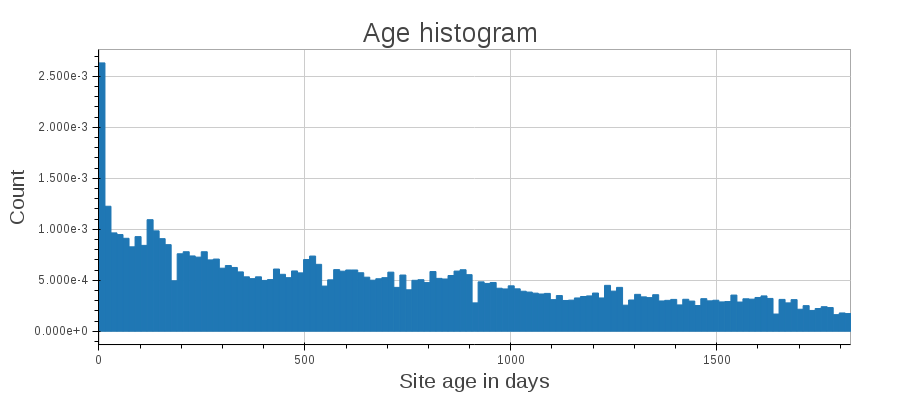
\includegraphics[scale=.18]{images/histogram_age}
        \end{center}
        \newline{}
        \begin{center}
            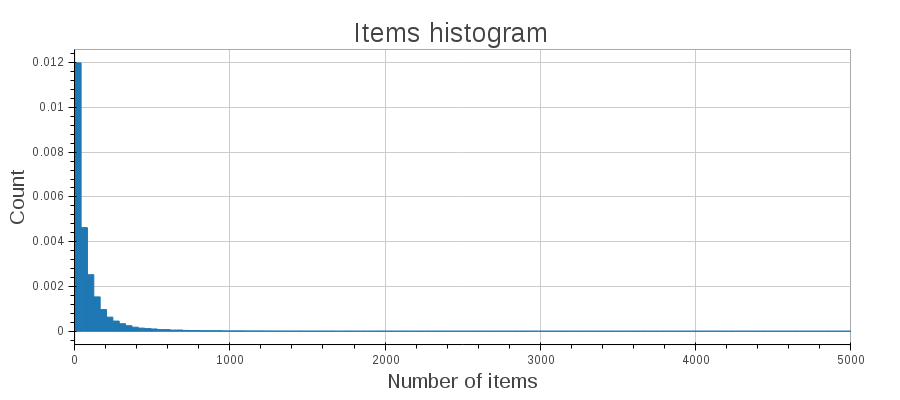
\includegraphics[scale=.18]{images/histogram_items}
        \end{center}
     \end{column}
    \end{columns}

\end{frame}


\begin{frame}[fragile]{Sales visualization}
    \begin{center}
        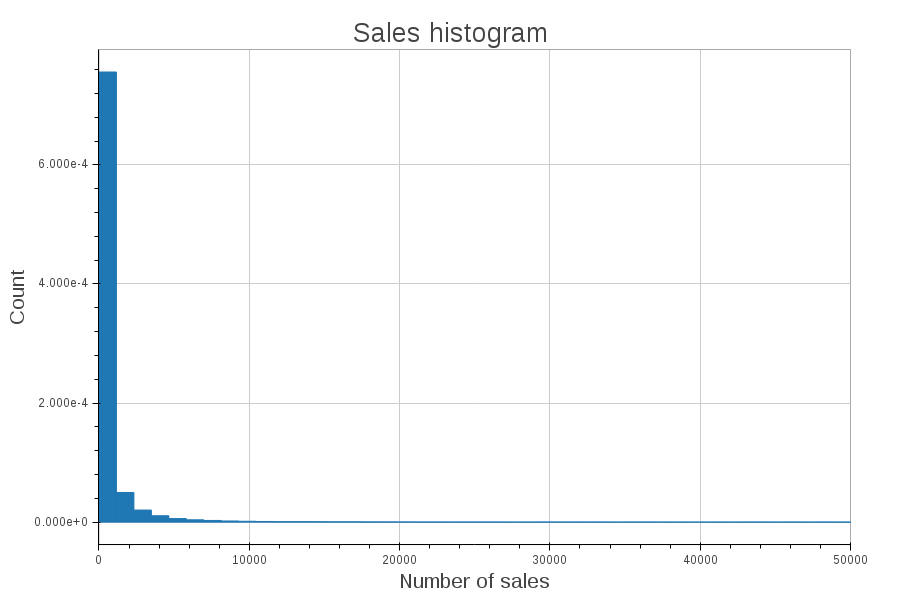
\includegraphics[scale=.25]{images/histogram_sales}
    \end{center}
\end{frame}


\begin{frame}[fragile]{Feature correlation}
    \begin{center}
        \begin{tabular}{lrrrrr}
        \toprule
        {} &     sales &  admirers &       age &  feedback &     items \\
        \midrule
        sales    &  1.000000 &  0.458261 &  0.181045 &  0.955949 &  0.502423 \\
        admirers &  0.458261 &  1.000000 &  0.340939 &  0.401995 &  0.268985 \\
        age      &  0.181045 &  0.340939 &  1.000000 &  0.184238 &  0.167535 \\
        feedback &  0.955949 &  0.401995 &  0.184238 &  1.000000 &  0.458955 \\
        items    &  0.502423 &  0.268985 &  0.167535 &  0.458955 &  1.000000 \\
        \bottomrule
        \end{tabular}
    \end{center}
\end{frame}


\begin{frame}[fragile]{Correlation to sales}
    \begin{columns}
     \begin{column}{.49\textwidth}
        \begin{center}
            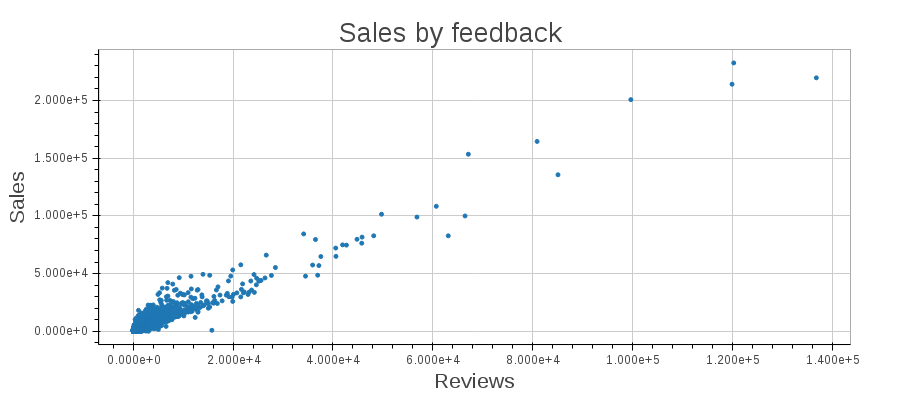
\includegraphics[scale=.18]{images/scatter_feedback}
        \end{center}
        \newline{}
        \begin{center}
            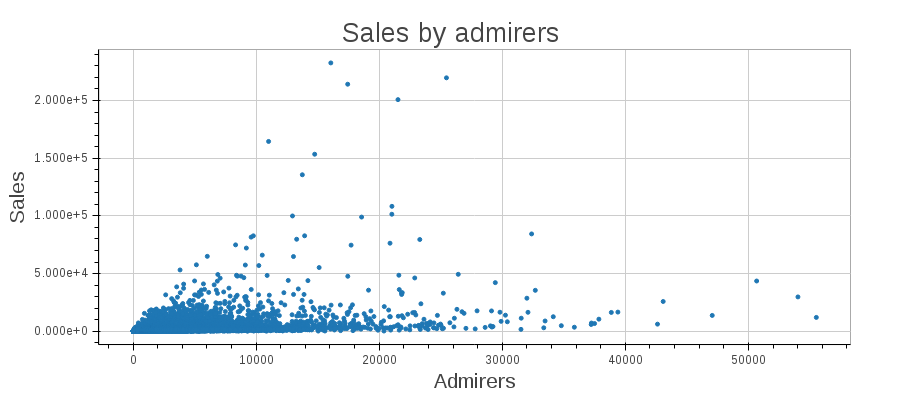
\includegraphics[scale=.18]{images/scatter_admirers}
        \end{center}
     \end{column}
    
     \begin{column}{.49\textwidth}
        \begin{center}
            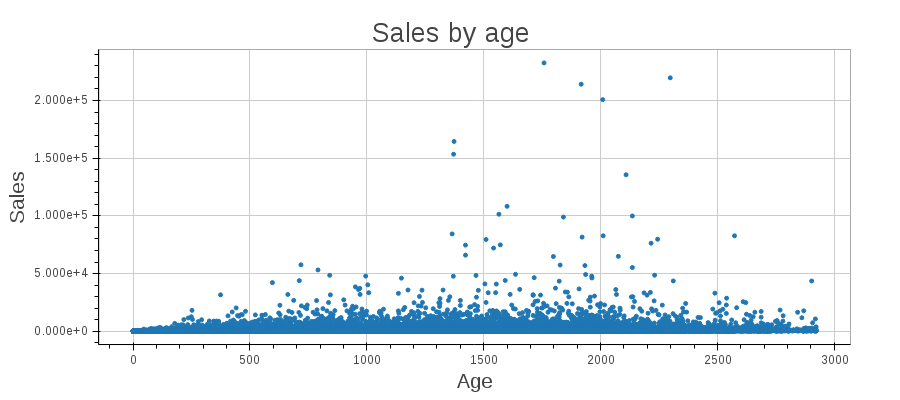
\includegraphics[scale=.18]{images/scatter_age}
        \end{center}
        \newline{}
        \begin{center}
            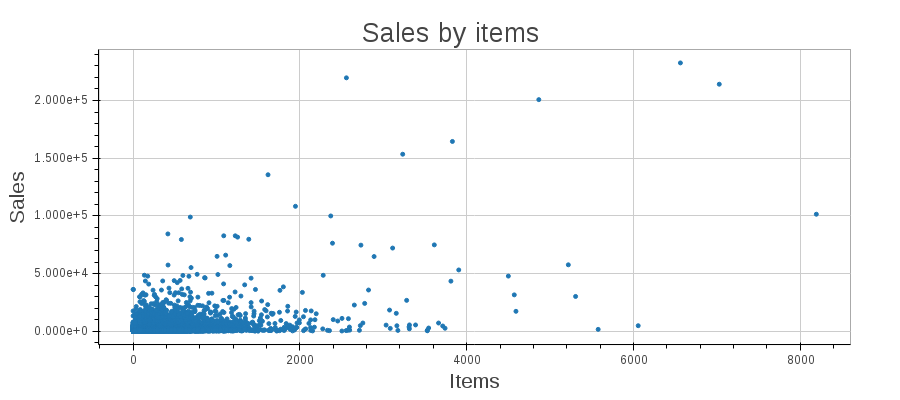
\includegraphics[scale=.18]{images/scatter_items}
        \end{center}
     \end{column}
    \end{columns}

\end{frame}

\begin{frame}[fragile]{Decision tree visualization}
    \begin{center}
        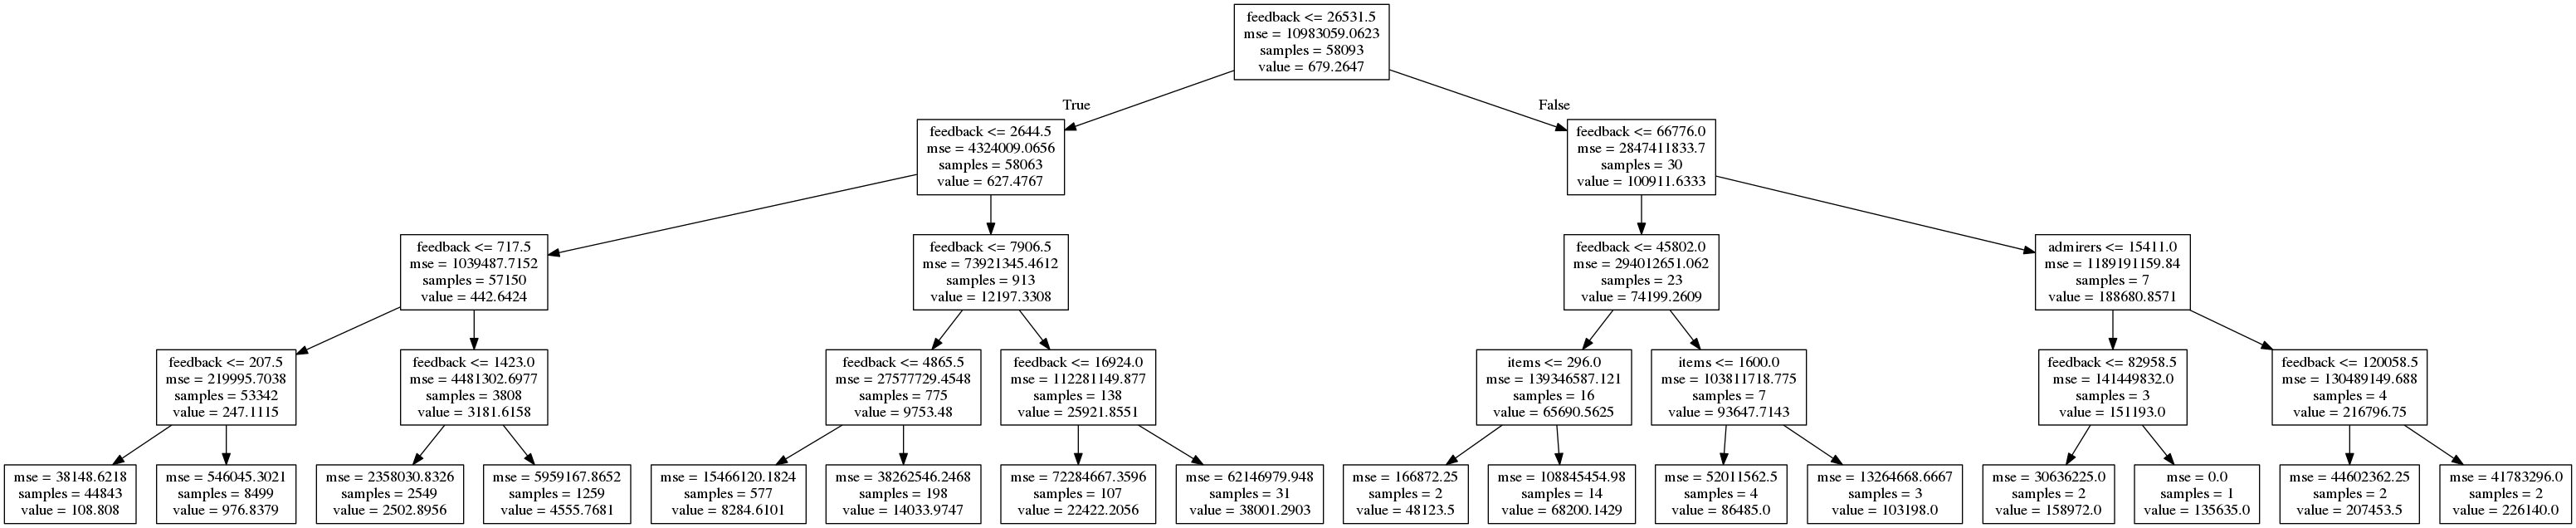
\includegraphics[scale=.13]{images/etsy_tree}
    \end{center}
\end{frame}

\begin{frame}[fragile]{Decision tree visualization (top)}
    \begin{center}
        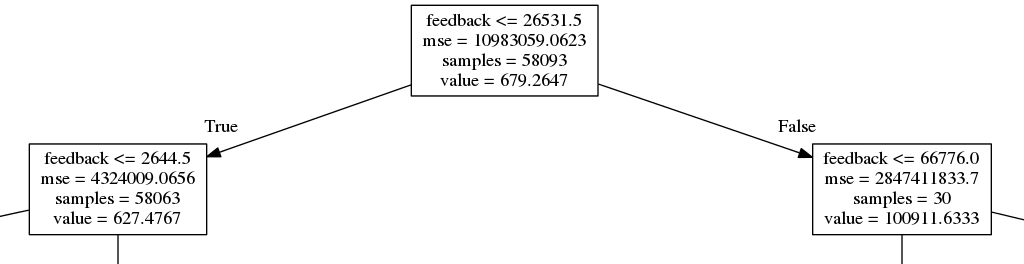
\includegraphics[scale=.40]{images/etsy_tree_top}
    \end{center}
\end{frame}

\begin{frame}[fragile]{Decision tree visualization (left)}
    \begin{center}
        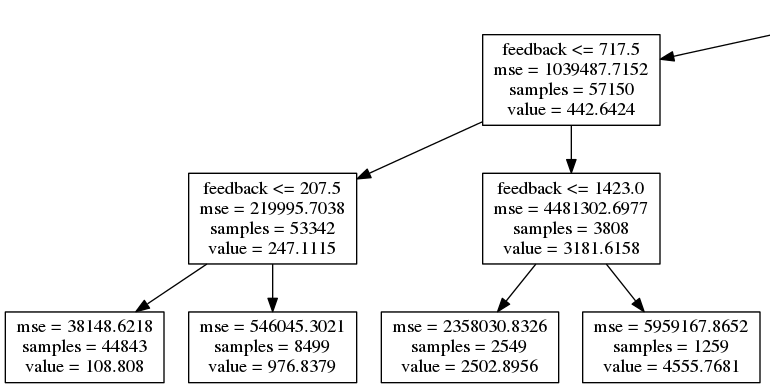
\includegraphics[scale=.40]{images/etsy_tree_left}
    \end{center}
\end{frame}

\begin{frame}[fragile]{Decision tree visualization (right)}
    \begin{center}
        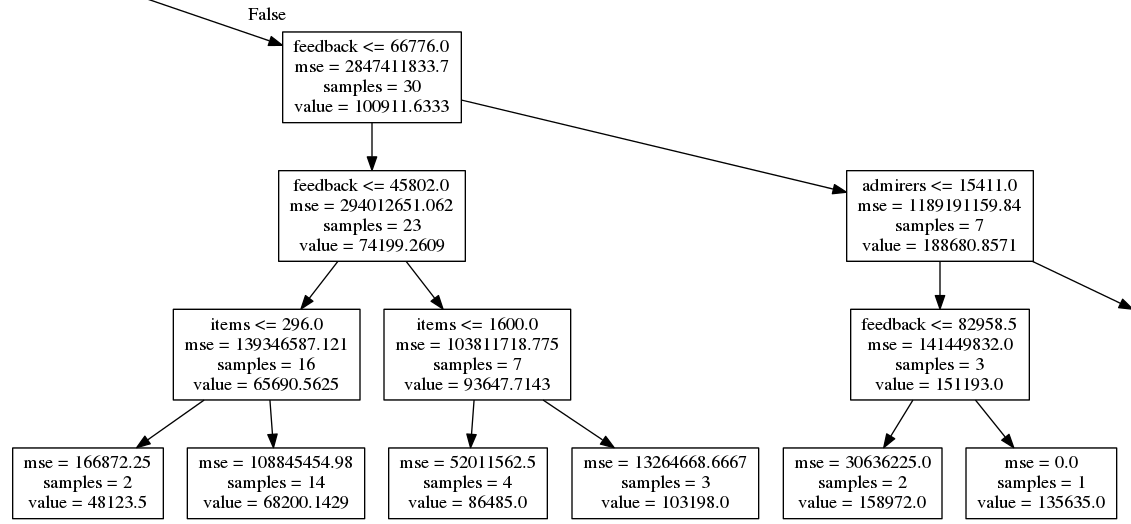
\includegraphics[scale=.30]{images/etsy_tree_right}
    \end{center}
\end{frame}

\begin{frame}[fragile]{What is wrong with the tree?}
    \begin{itemize}
        \item Only \textbf{one variable} used to predict in some cases
        \item Lack of \textbf{stability}:
        \begin{itemize}
            \item If feedback = 207 we predict 109 sales
            \item If feedback = 208 we predict 977 sales
            \item Our model can change dramatically if we add few more samples to the dataset
        \end{itemize}
        \item \textbf{Overfitting}: We make predictions based on a single sample
    \end{itemize}

\end{frame}

\section{Training Random Forests}

\begin{frame}{Ensembles: The board of directors}
    \begin{columns}
     \begin{column}{.49\textwidth}
        \begin{itemize}
            \item Why companies have a BoD?
            \item What is best?
            \begin{itemize}
                \item The best point of view
                \item A mix of good points of view
            \end{itemize}
            \newline{}
            \item How was our best tree?
            \begin{itemize}
                \item What about a mix of not so good trees?
            \end{itemize}

        \end{itemize}

     \end{column}
    
     \begin{column}{.49\textwidth}
        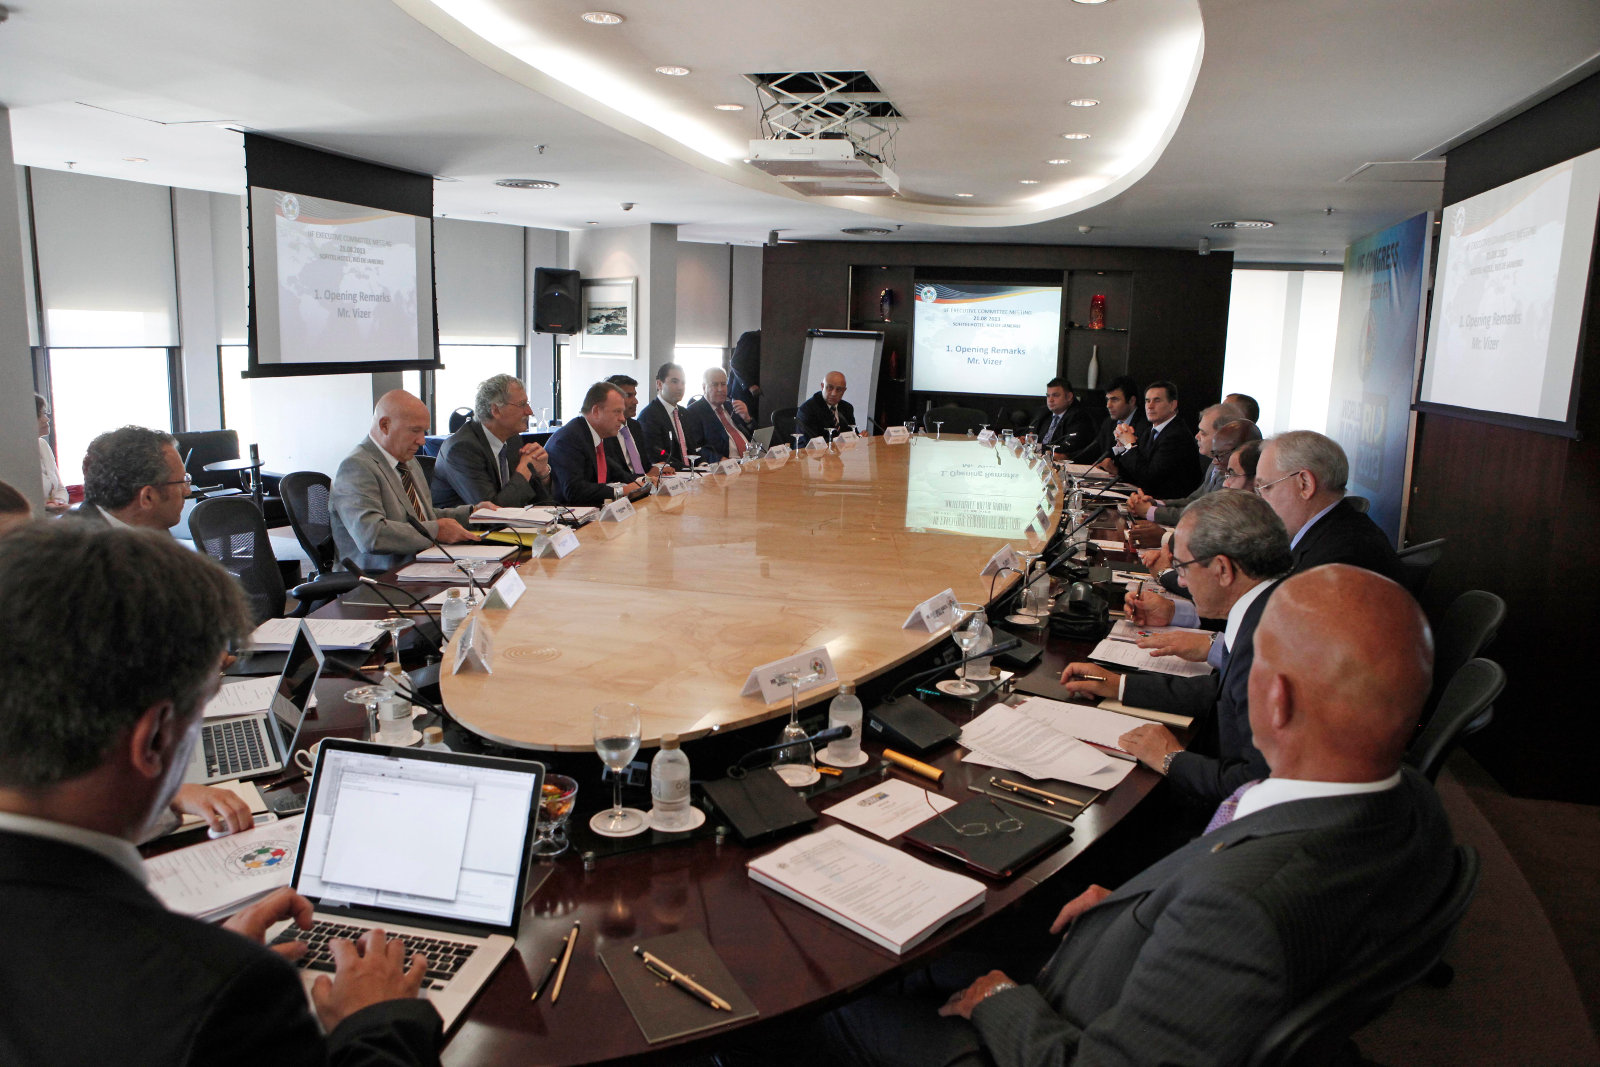
\includegraphics[scale=.12]{images/bod}
     \end{column}
    \end{columns}
\end{frame}

\begin{frame}[fragile]{Ensemble of trees}
    \begin{itemize}
        \item How do we build optimized trees, that are different?
        \begin{itemize}
            \item We need to \emph{randomize} them
            \begin{itemize}
                \item Samples: bagging
                \item Features
                \item Splits
            \end{itemize}
        \end{itemize}
    \end{itemize}
\end{frame}

\begin{frame}[fragile]{Bagging: Uniform sampling with replacement}
    \begin{columns}
     \begin{column}{.49\textwidth}
        \begin{center}
            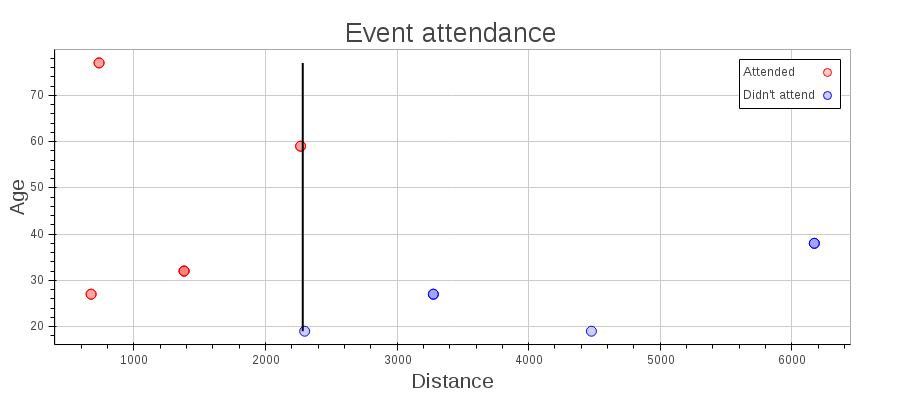
\includegraphics[scale=.18]{images/bagging1}
        \end{center}
        \newline{}
        \begin{center}
            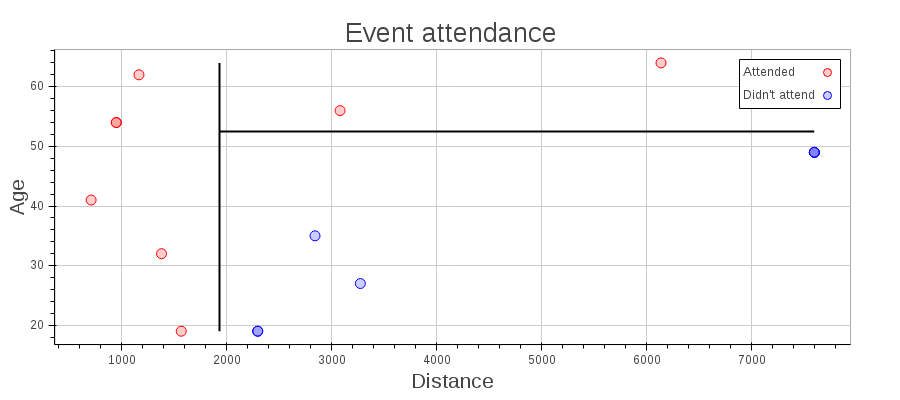
\includegraphics[scale=.18]{images/bagging2}
        \end{center}
     \end{column}
    
     \begin{column}{.49\textwidth}
        \begin{center}
            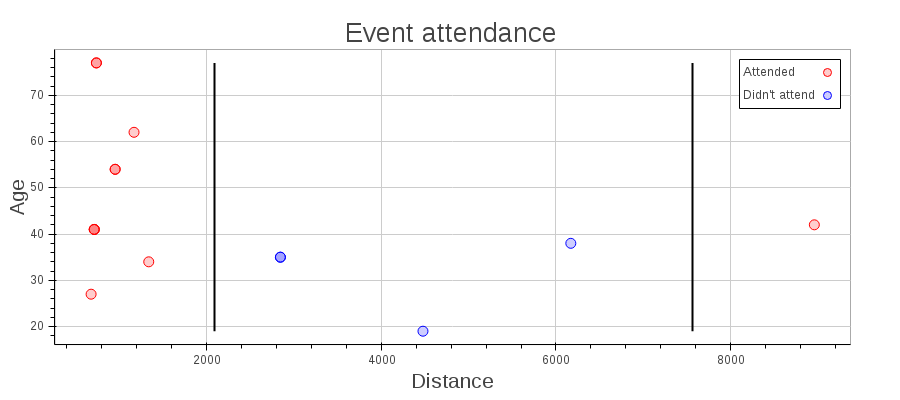
\includegraphics[scale=.18]{images/bagging3}
        \end{center}
        \newline{}
        \begin{center}
            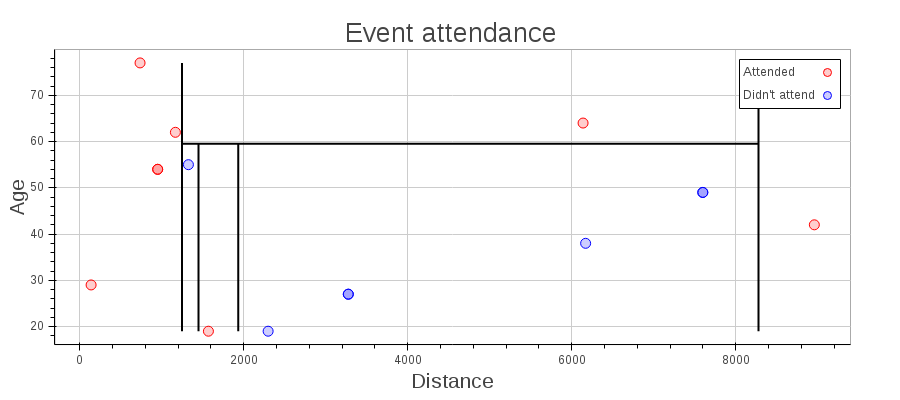
\includegraphics[scale=.18]{images/bagging4}
        \end{center}
     \end{column}
    \end{columns}
\end{frame}

\begin{frame}{Randomizing features}
    \begin{itemize}
        \item Even with bagging, trees will usually make the top splits by the same feature
        \item \emph{max\_features} parameter:
        \begin{itemize}
            \item Regression: Use all
            \item Classification: Use the squared root
        \end{itemize}
    \end{itemize}

\end{frame}

\begin{frame}{Randomizing splits}
    \begin{itemize}
        \item A split per sample is considered in the original decision tree
        \item We can consider a subset
        \begin{itemize}
            \item We obtain randomized trees
            \item Performance is improved
        \end{itemize}
        \item \emph{sklearn} implements \textbf{ExtraTreeRegressor} and \textbf{ExtraTreeClassifier}
    \end{itemize}

\end{frame}


\begin{frame}[fragile]{What happened with our example problems}
    \begin{itemize}
        \item Only \textbf{one variable} used to predict in some cases
        \begin{itemize}
            \item \emph{We can avoid it by not using all features}
        \end{itemize}
        \item Lack of \textbf{stability}:
        \begin{itemize}
            \item \emph{Our model is smoother}
        \end{itemize}
        \item \textbf{Overfitting}: We make predictions based on a single sample
        \begin{itemize}
            \item \emph{Overfitting is mostly avoided}
            \item Random forests come with built-in cross validation
        \end{itemize}

    \end{itemize}

\end{frame}

\begin{frame}[fragile]{Smoothing}
    \begin{center}
        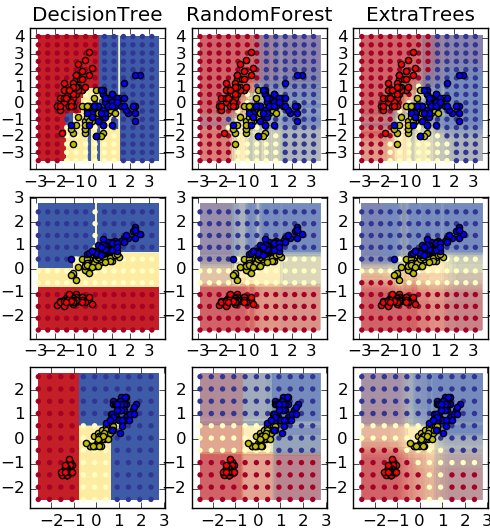
\includegraphics[scale=.40]{images/plot_forest_iris_001}
    \end{center}
\end{frame}

\begin{frame}[fragile]{Parameter optimization (Etsy)}
    \begin{center}
        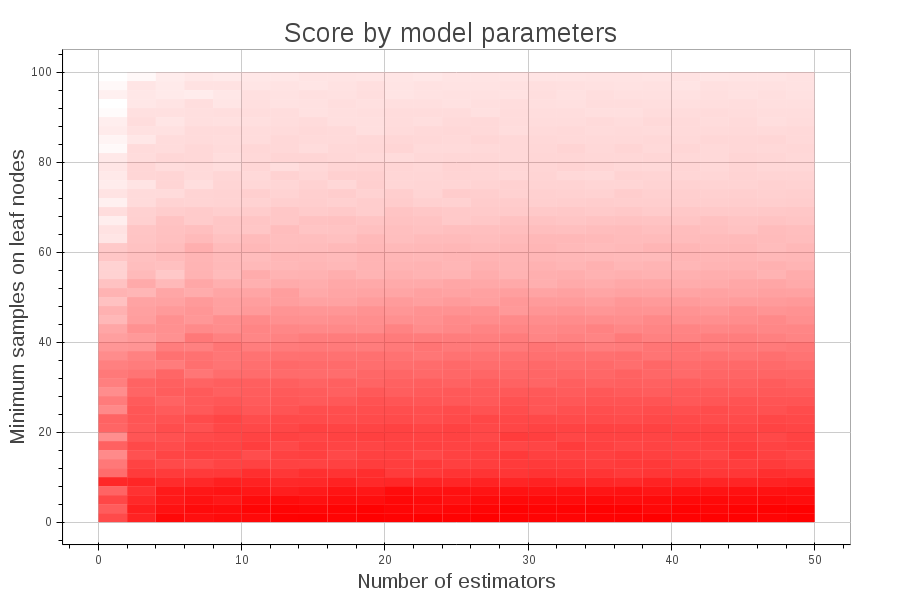
\includegraphics[scale=.25]{images/heatmap_nestim_minsamp}
    \end{center}
\end{frame}

\begin{frame}[fragile]{Parameter optimization (Bank marketing)}
    \begin{center}
        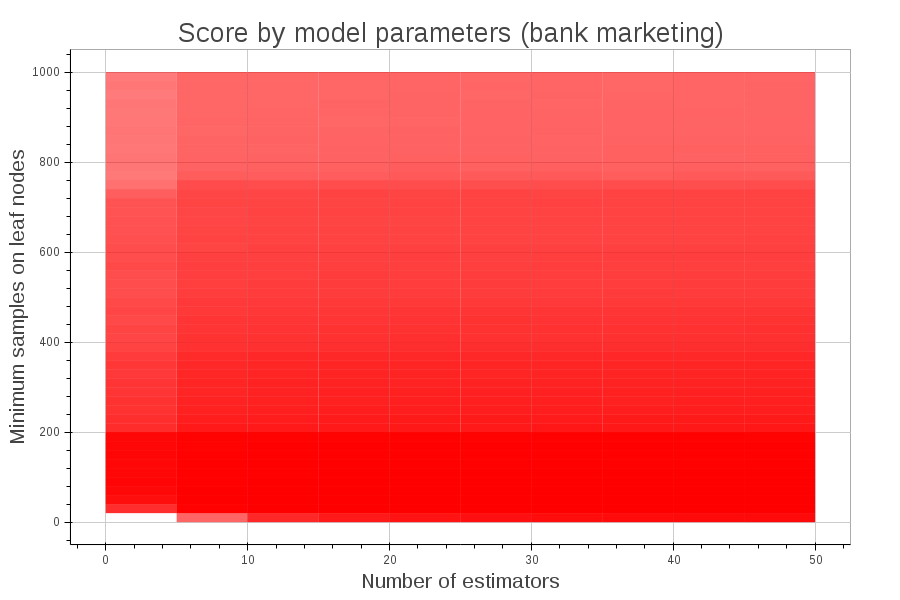
\includegraphics[scale=.22]{images/heatmap_nestim_minsamp_bankmkt}
    \end{center}
    \tiny{Data source: [Moro et al., 2014] S. Moro, P. Cortez and P. Rita.\newline{}
    A Data-Driven Approach to Predict the Success of Bank Telemarketing. Decision Support Systems, Elsevier, 62:22-31, June 2014}
\end{frame}

\begin{frame}[fragile]{When should we use Random Forests?}
    \begin{itemize}
        \item Using a CART is usually good as part of exploratory analysis
        \item Do \emph{not} use CART or RF when the problem is linear
        \item They are specially good for ordinal (categorical but sorted) variables
        \item Performance
        \begin{itemize}
            \item CART is slower than linear models (e.g. logit)
            \item RF trains N trees, and takes N times \textbf{but it works in multiple cores, seriously}
            \item But RF is usually much faster than ANN or SVM, and results can be similar
        \end{itemize}
    \end{itemize}

\end{frame}

\begin{frame}[fragile]{Summary}
    \begin{itemize}
        \item CART is a simple, but still powerful model
        \begin{itemize}
            \item Visualizing them we can better understand our data
        \end{itemize}
        \item Ensembles usually improve the predictive power of models
        \item Random Forests fix CART problems
        \begin{itemize}
            \item Better use of features
            \item More stability
            \item Better generalization (RFs avoid overfitting)
        \end{itemize}
        \item Random Forests main parameters
        \begin{itemize}
            \item min\_samples\_leaf (inherited from CART)
            \item num\_estimators
        \end{itemize}

    \end{itemize}

\end{frame}

\begin{frame}[fragile]{Thank you}
    \begin{center}
        \Large
        QUESTIONS?
    \end{center}

\end{frame}

\end{document}


%%% Local Variables:
%%% mode: latex
%%% TeX-master: "demo-slides.tex"
%%% End:
